\section{Ejercicio 1: Vamos a buscar la respuesta a P=NP!}
    % 1. Describir detalladamente el problema a resolver dando ejemplos del mismo y sus soluciones.
    \subsection{Descripción del problema}
		\begin{figure}[ht]
			\begin{center}
				
\includegraphics[width=0.5\columnwidth]{imagenes/expedicionistas.jpg}
				\caption{Indiana Jones junto a un Canibal del grupo de exploración}
			\end{center}
		\end{figure}
        Indiana Jones debe seguir un mapa que posiblemente lo lleve a encontrar la solución a P=NP. Para esto, lleva a un grupo de arquéologos compuesto por $A$ personas y le pide ayuda a un grupo de gente local de tamaño $C$ para poder llegar hasta su destino sin grandes problemas. Sin embargo, durante el camino se encuentran con un puente en mal estado en el que no podrán pasar más de dos personas a la vez. Sumado a eso, hay solo una linterna para todo el equipo, por lo que en cada cruce alguien debe volver con la linterna. Como si el problema del puente fuera poco, el grupo local es conocido por su canibalismo, así que no pueden quedar más caníbales que arqueólogos de alguno de los lados del puente.

        La resolución del problema consiste en elaborar un programa que recibe como entrada el valor de $A$ y $C$, y luego las velocidades de cada arqueólogo ($a_0, ... , a_A$) y la de cada canibal ($c_0, ... , c_C$) y devuelve la velocidad mínima con la que se puede cruzar el puente.

        Por ejemplo, si el programa recibe lo siguiente como entrada: \newline
        \texttt{2} \texttt{1} \newline
        \texttt{1} \texttt{2} \newline
        \texttt{1}

        La salida correcta sería: \newline
        \texttt{4}

    % 2. Explicar de forma clara, sencilla, estructurada y concisa, las ideas desarrolladas para la resolución del problema. Utilizar pseudocódigo y lenguaje coloquial (no código fuente). Justificar por qué el procedimiento resuelve efectivamente el problema.
    \subsection{Solución propuesta}
        La solución de este problema fue lograda considerando todos las formas posibles de cruzar el puente. Para esto, el algoritmo propuesto chequea todas las posibilidades que se tienen para ir de un lado al otro del puente. Es decir, sea $A1$, $A2$ y $C1$, $C2$ dos personas de cada grupo, se elige una de las formas que hay de cruzar el puente, las cuales consisten en que cruce alguno de los elementos \{A1, C1, (A1,C1), (A1,A2), (C1,C2)\}. Para cada una de esas opciones, se intentara realizar el cruce $\forall a \in$ \emph{arqueólogos} y $\forall c \in$ \emph{caníbales}. En otras palabras, se realiza el intento para todas las combinaciones de personas que hay.

        Además, lo que tomamos como velocidad en cada cruce es el tiempo que tarda pasar un grupo o persona desde un lado del puente a otro. Es decir, sean $C =\{c1,c2,c3\}$, conjunto de caníbales y sea $A =\{a1,a2,a3\}$ de arqueólogos, cada uno con su respectiva velocidad. Sean $x,y\in$C$\cup$A. Entonces la velocidad de pasar x e y es del max(V(x), V(y)) con V la funcion que da la velocidad de una persona.

        Solamente van a tener la chance de cruzar quienes estén del lado en que está en la linterna y que su cruce no lleve a un \emph{estado inválido}. Un estado válido es aquél en el que no se estuvo anteriormente (con respecto a la cantidad de caníbales y arqueólogos de cada lado y a la ubicación de la linterna) y que no deje a más caníbales que arqueólogos de alguno de los dos lados.

        Una solución es válida cuando lograron cruzar todos las personas (arqueólogos y caníbales) de un lado al otro del puente. Esto es posible si no hubo estados inválidos en el camino para que todos crucen. Dado que se prueban todas las combinaciones posibles, vamos a obtener múltiples soluciones de distintas velocidades. Es por ello que una vez que se tengan todos las soluciones posibles, se compararán las velocidades de cada solución y se tomará la mínima.

        Teniendo en cuenta lo planteado en este informe sobre el problema, podemos marcar que el algoritmo realizado fue construido en base a la técnica de \emph{backtracking} que al igual que en este caso, consiste en probar todas las posibilidades descartando la mayor cantidad de soluciones incorrectas posibles al mismo tiempo y dejando como resultado una lista con las soluciones válidas. Así, se prueban todos los caminos posibles para cruzar el puente y al final se obtiene una lista con todos los tiempos que puede tomar cruzar el puente (excepto el caso donde no haya ningún caso posible, que devolvemos -1).

        Más específicamente, la aplicación de \emph{backtracking} en este problema consiste en probar todos los idas y vueltas de todas las combinaciones de personas, pero sumado a que la poda utilizada es la de no repetir estados, cuya correctitud será explicada posteriormente. El algoritmo tiene forma recursiva que depende de la cantidad de arqueólogos y caníbales de cada lado y la unicación de la linterna (al igual que la validez de los estados).

        El caso base de la recursión es la que hay 0 arqueólogos y 0 caníbales del lado de izquierdo momento en el cual la iteración finaliza al agregar el tiempo acumulado hasta el momento en la lista de soluciones. Este tiempo acumulado corresponde a la suma de velocidadades con las que se cruzó el puente cada vez.

        Para el caso recursivo, se chequeará antes de entrar en la recursión que el estado al que se va a cambiar sea uno válido. Si no lo es, cambia la cantidad de exploradores que vayan a cruzar entre alguna de las 5 posibilidades antes mencionadas. Si siguen obteniéndose estados inválidos, entonces no quedarán casos para probar y simplemente terminará la búsqueda sin haber encontrado una solución válida. Si venía de una recursión, entonces el algoritmo probara con otro estado en el punto anterior. Si no, termina el algoritmo.

    \begin{codesnippet}
    \begin{verbatim}

    BTCruzarPuentes(Parámetros)
    si estadoActual tiene linterna a la derecha
      lado de origen  = lado derecho
      lado de destino = lado izquierdo
    si no
      lado de origen  = lado izquierdo
      lado de destino = lado derecho
    linternaEnDeracha = !linternaEnDerecha
    
    esSolucion = canibales_izq + arquielogos_izq == 0;
    Si es solucion
        encolar tiempo en soluciones
    } sino    


        for #mandarCanibales = 0 ... minimo(2, #canibales del lado de origen):
          for #mandarArqueologos = 0 ... (2 - #CanibalesQueCruzan):
            if esEstadoValido(#CanibalesEnOrigen - #canibalesQueCruzan,
                              #ArqueologosEnOrigen - #arqueologosQueCruzan,
                              #CanibalesEnDestino + #CanibalesQueCruzan,
                              #ArqueologosEnDestino + #ArqueologosQueCruzan,
                              linternaEnDerecha, estadosAnteriores):
              

              
              switch((#mandarCanibales,#mandarArqueologos)
                  moverEsaCantidad
                  cambiarDeLadoLinterna
                  guardarEstadoNuevo
                  BTCruzarPuente
              end switch

            endif  
          end for
        end for
      end if
    \end{verbatim}
    \end{codesnippet}

            Esta es una parte del pseudocódigo del algoritmo completo, en la cual se muestra cómo funciona la parte recursiva del mismo. Esta función, toma como parámetros de entrada \emph{&canibalesOrigen, &arqueologosOrigen, &canibalesDestino, &arqueologosDestino,linternaDer, &estadosAnteriores, tiempo, &soluciones}. 


            El algoritmo, en primer lugar chequea si dentro del estado en el cual entró a la recursión, cruzaron todos los exploradores (arqueólogos y caníbales). En tal caso, se agrega el \emph{tiempo} que tomó cruzar el puente a la variable \emph{soluciones}. 
            Luego, regresa de la recursión para volver hacia arriba en un nivel en el árbol de ejecución y se continúa probando las otras posibilidades de caminos.

            Caso contrario, el algoritmo prueba todos los casos de mandar caníbales y/o arqueólogos por el puente (tomando en cuenta de mandar uno solo o dos). Por cada caso, si el movimiento es válido, entrará a una función correspondiente a mover esa cantidad de tales grupos. Esta función mencionada, es la encargada de mover la linterna, crear un nuevo estado, y junto con este nuevo estado, prueba por cada explorador, mandar a todos los que estén disponibles. 


            Entonces, cada vez que un explorador es elegido, se crea un nuevo estado y es agregado a un vector de \textbf{estados}. La idea de agregar nuevoEstado a EstadosAnteriores consiste en poder eliminar los caminos que lleven a una situación que ya se haya estado con anterioridad (por ejemplo, que cruce un canibal y luego vuelva), para evitar loops infinitos. Además, al quitarla luego de la recursión hace que para cada altura del árbol de ejecución tengamos la misma cantidad de estados y que éstos sean todos distintos. La razón por la cual serán distintos proviene de que cada estado se arma basándose en la cantidad de arqueólogos y caníbales que hay de cada lado y luego sus velocidades, según de qué lado está la linterna. Entonces si cada vez que haya que cruzar el puente se elige una cantidad distinta de exploradores, cada nuevo estado tendrá como máximo 5 formas distintas (que cruce un solo canibal, un solo arqueólogo, dos canibales, dos arqueólogos o un arqueólogo y un canibal). Y por cada tipo de explorador elegido, se entra a la recursión con cada uno de los que se encuentran del lado de la linterna.

            Finalmente, se devuelve el vector de \emph{soluciones}, el cual contiene cada uno de los tiempos, y se devuelve el mínimo.



          







        \subsubsection{Detalles implementativos}
            El algoritmo fue implementado en lenguaje C++. Para almacenar la solución, se recurre a la clase \texttt{vector}, proporcionada por la librería estándar del lenguaje.

            Para manejar los estados en el árbol de ejecución, se van almacenando los nuevos estados en un vector de \texttt{Estados} antes de entrar en una recursión y se quita al retornar de la misma. Esto es para que, si del estado $S_{i}$, se agrega un estado y se llega al $S_{i+1}$, si este es inválido, pueda regresar nuevamente a $S_{i}$, e intentar con otros estados. Además, esto sirve para que para el mismo nivel dentro del árbol de recursión, la cantidad de estados dentro de cada nodo interno u hoja, sea la misma.

            Un \texttt{Estado} es una clase la cual consiste de 4 \texttt{Int}, 2 para la cantidad de arqueólogos y 2 para la cantidad de caníbales de cada uno de los lados en ese momento, y de un \texttt{Bool} para indicar si la linterna se encuentra a la derecha o no.

            Llamamos \emph{árbol de ejecución} al árbol que se va generando de acuerdo a las desiciones tomadas en cuanto a qué explorador cruzará el puente.

            La forma en que se elige quiénes cruzarán de un lado a otro luego de haber decidido a qué grupo pertenecen, es simplemente tomar los primeros (1 o 2) valores del vector que contiene a los arqueólogos o caníbales que vayan a pasar. De esta forma se están tomando siempre los más rápidos, como se mencionó anteriormente, ya que en cada iteración los 4 vectores de personas se ordenan de menor a mayor.


    \subsection{Demostración de la correctitud}
      Para demostrar correctitud del algoritmo debemos demostrar por un lado, que utilizar la técnica backtracking cumple que recorre todos los casos y devuelve el más rápido. Y por otro lado que las podas de que siempre sean los más rapidos y de evitar que se repitan casos son válidas.
      Esto último se puede ver dentro del algoritmo. Pues por cada nuevo estado, es guardado en un struct \emph{Estados}, luego el mismo es usado como parámetro para la función \emph{estadoValido}, el cual chequea en un vector de estadosAnteriores, si a ese estado ya se llegó. Si esto pasa, el algoritmo prueba mandar otro/s arqueólogo/s o caníbal/es según toque en el ciclo principal para encontrar un nuevo estado.\par

      Por otro lado, vamos a demostrar  



    % 3. Deducir una cota de complejidad temporal del algoritmo propuesto y justificar por qué el algoritmo cumple la cota dada. Utilizar el modelo uniforme.
    \subsection{Complejidad teórica}

      El algoritmo comienza tomando $2$ vectores ($arqs$ y $cani$), siendo uno para los arqueólogos y otro para los caníbales. En cada posición de $arqs$ y $cani$ se encontrará una velocidad correspondiente a algún arqueólogo o caníbal. El tamaño de cada vector será igual a la cantidad de arqueólogos/caníbales que se tomaron como entrada. Llamaremos $n$ a la cantidad de arqueólogos. Además, dada la lógica del algoritmo, si hay más caníbales que arqueólogos al comenzar, la ejecución termina sin llamar a la función principal y devuelve $-1$ inmediatamente, ya que no hay forma de que al comienzo haya más arqueólogos que caníbales en el lado izquierdo. En cambio, si hay $0$ aqrueólogos o más arqueólogos que caníbales, sí se llama a la función que realiza \emph{Backtracking}.
      En ella, se utilizan $2$ vectores más para poder distinguir el lado del que se encuentra cada arqueólogo y cada caníbal. La inserción y eliminación de cada elemento en cada vector será de $O(1)$ amortizado ya que en caso de que el vector deba redimencionarse, se copian todos los elementos del vector a uno más grande dejando como complejidad $O(n)$.
      En cada llamada a la función principal del algoritmo, se prueban $5$ casos: que cruce un arqueólogo solo, un canibal solo, dos arqueólogos, dos caníbales o un caníbal y un arqueólogo. Luego, cada nodo del árbol tendrá 5 hijos. Cada uno de ellos, será un posible estado válido, que se chequea revisando un vector de \emph{estados válidos}, que a lo sumo tendrá el tamaño de la altura del árbol a causa de mantener todos los estados válidos anteriores a cada nodo, y por lo tanto tomará $O(n^2)$ (probado más adelante). Si es un estado válido, se realizarán las operaciones necesarias para decidir quién cruzará el puente, las cuales consisten en los movimientos de personas entre vectores (que toma complejidad $O(n)$), previamente habiendo ordenado cada vector (en $O(n $log$ n)$) y luego llamar recursivamente a la función principal, lo que da una complejidad de $O(n^2)$ para las operaciones que no son la llamada recursiva. Dado que se quieren probar todos los estados válidos, podemos decir que la complejidad temporal será el tiempo que tome recorrer cada uno de estos estados, que a la vez equivalen a los nodos del árbol de ejecución. Como fue mencionado en la sección de \textbf{Solución Propuesta}, en caso de haber un caso inválido, este es descartado para probar otros casos posibles es decir la altura del árbol está acotada por la cantidad total de estados válidos. Este número se calcula de la siguiente manera:

      Dado que la cantidad de caníbales está acotada por la cantidad de arqueólogos, la cantidad de formas válidas que hay para repartir a todas las personas en ambos lados del puente manteniendo el invariante de que no haya más caníbales que arqueólogos de ninguno de los dos lados se calcula utilizando combinatoria. La cantidad de caníbales posibles en cada lado del puente es menor o igual a la cantidad de arqueólogos de ese lado (o sea entre $0$ y $n$), pero en caso de que no haya arqueólogos en alguno de los lados, la cantidad de caníbales posibles es igual a la cantidad total de arqueólogos, salvo que no haya ninguno y en ese caso $n$ pasará a ser el número de caníbales totales.

      \[
      \sum_{i=1}^{n}(i+1) + (n+1)
      \]
      \[
      \frac{(n+2)(n+1)}{2} + (n+1) - 1
      \]
      \[
      \frac{(n+2)(n+1)}{2} + n
      \]
      \[
      \frac{(n+2)(n+1)+2n}{2}
      \]
      \[
      \frac{n^2+3n+2}{2}
      \]

      Y de este tipo de funcion sabemos \newline

      \[
      \frac{n^2+3n+2}{2} \in O(n^2)
      \]

      Entonces, la altura del árbol va a estar acotada por $O(n^2)$.
      Retomando, llegamos a que la complejidad de encontrar las soluciones está acotada por $O(b^h)$ donde $b$ es la cantidad de ramas que se abren en cada nodo, $h$ es la altura del árbol y todo esto es el tamaño del árbol. Como mencionamos anteriormente, $b$ es exactamente $5$ y la altura del árbol está acotada por $O(n^2)$. Luego, la complejidad temporal para encontrar las soluciones sería $O(5^{n^2})$. Pero hasta aquí no tenemos en cuenta que cada nodo cuesta $O(n^2)$. Incorporando esto a la complejidad anterior en la cual suponíamos que cada nodo tenía costo $O(1)$, nos queda que la complejidad temporal en peor caso es $O(n^2 * 5^{n^2})$.

      En cuanto a la complejidad espacial, se utiliza un historial de estados anteriores en los que se van guardando los estados válidos por los que se pasó hasta cierto punto en cada nodo del árbol. Se usa como si fuera una pila y cada vez que se accede a un nivel inferior en el árbol de ejecución, se guarda el estado actual de los caníbales, los arqueólogos y la linterna; mientras que cuando se sube en el árbol, se elimina el último estado actual. Debido a esto, la complejidad espacial en es $O(n^2)$ ya que la pila tendrá a lo sumo el mismo tamaño que la cantidad de estados en la rama más larga, y como probamos antes, este valor está acotado por esa complejidad. Además, lo que se guarda en cada estado son 4 valores enteros que indican la cantidad de arqueólogos y caníbales de cada lado, y un booleano (representado con 1 o 0) que indica de qué lado está la linterna.


    % 4. Dar un código fuente claro que implemente la solución propuesta. Se deben incluir las partes relevantes del código como apéndice del informe impreso entregado.

    % 5. Realizar una experimentación computacional para medir la performance del programa implementado. Usar un conjunto de casos de test en función de los parámetros de entrada, con instancias aleatorias e instancias particulares (de peor/mejor caso en tiempo de ejecución, por ejemplo). Presentar en forma gráfica una comparación entre los tiempos medidos y la complejidad teórica calculada y extraer conclusiones.
    \subsection{Experimentación}

	Para poder visualizar que la cota propuesta en la complejidad temporal funciona para el algoritmo que resuelve este problema, realizamos experimentos con entre 1 y 7 arqueólogos y caníbales, pero siempre con mayor o igual número de los primeros que de los segundos. Los casos de prueba pueden observarse en la tabla que se encuentra en el anexo de este informe.

  Los resultados obtenidos fueron plasmados en el siguiente gráfico. El mismo es la representación del tiempo en funcion de la cantidad de arqueólogos. También se muestra la funcion propuesta como cota de complejidad temporal.

  \begin{figure}[H]
      \begin{center}
        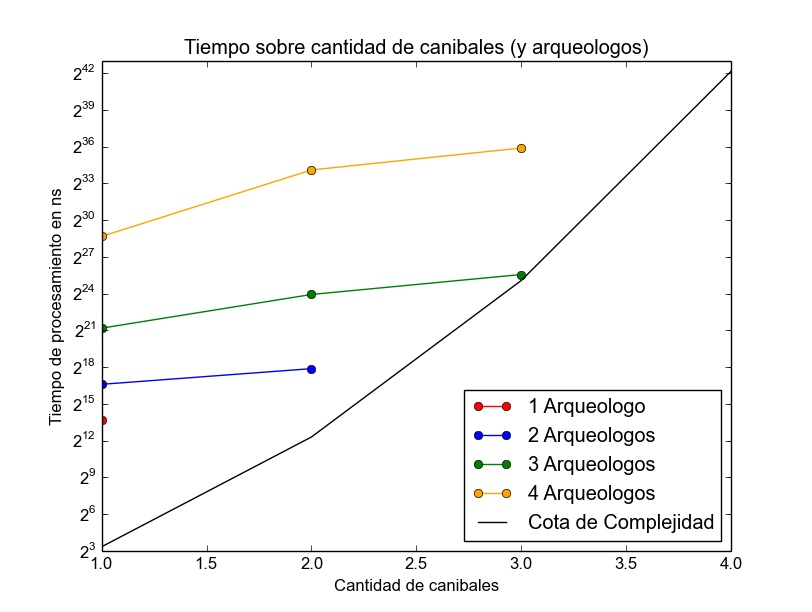
\includegraphics[width=1.1\columnwidth]{imagenes/ej1exp1NuevaVersion.jpeg}
        % 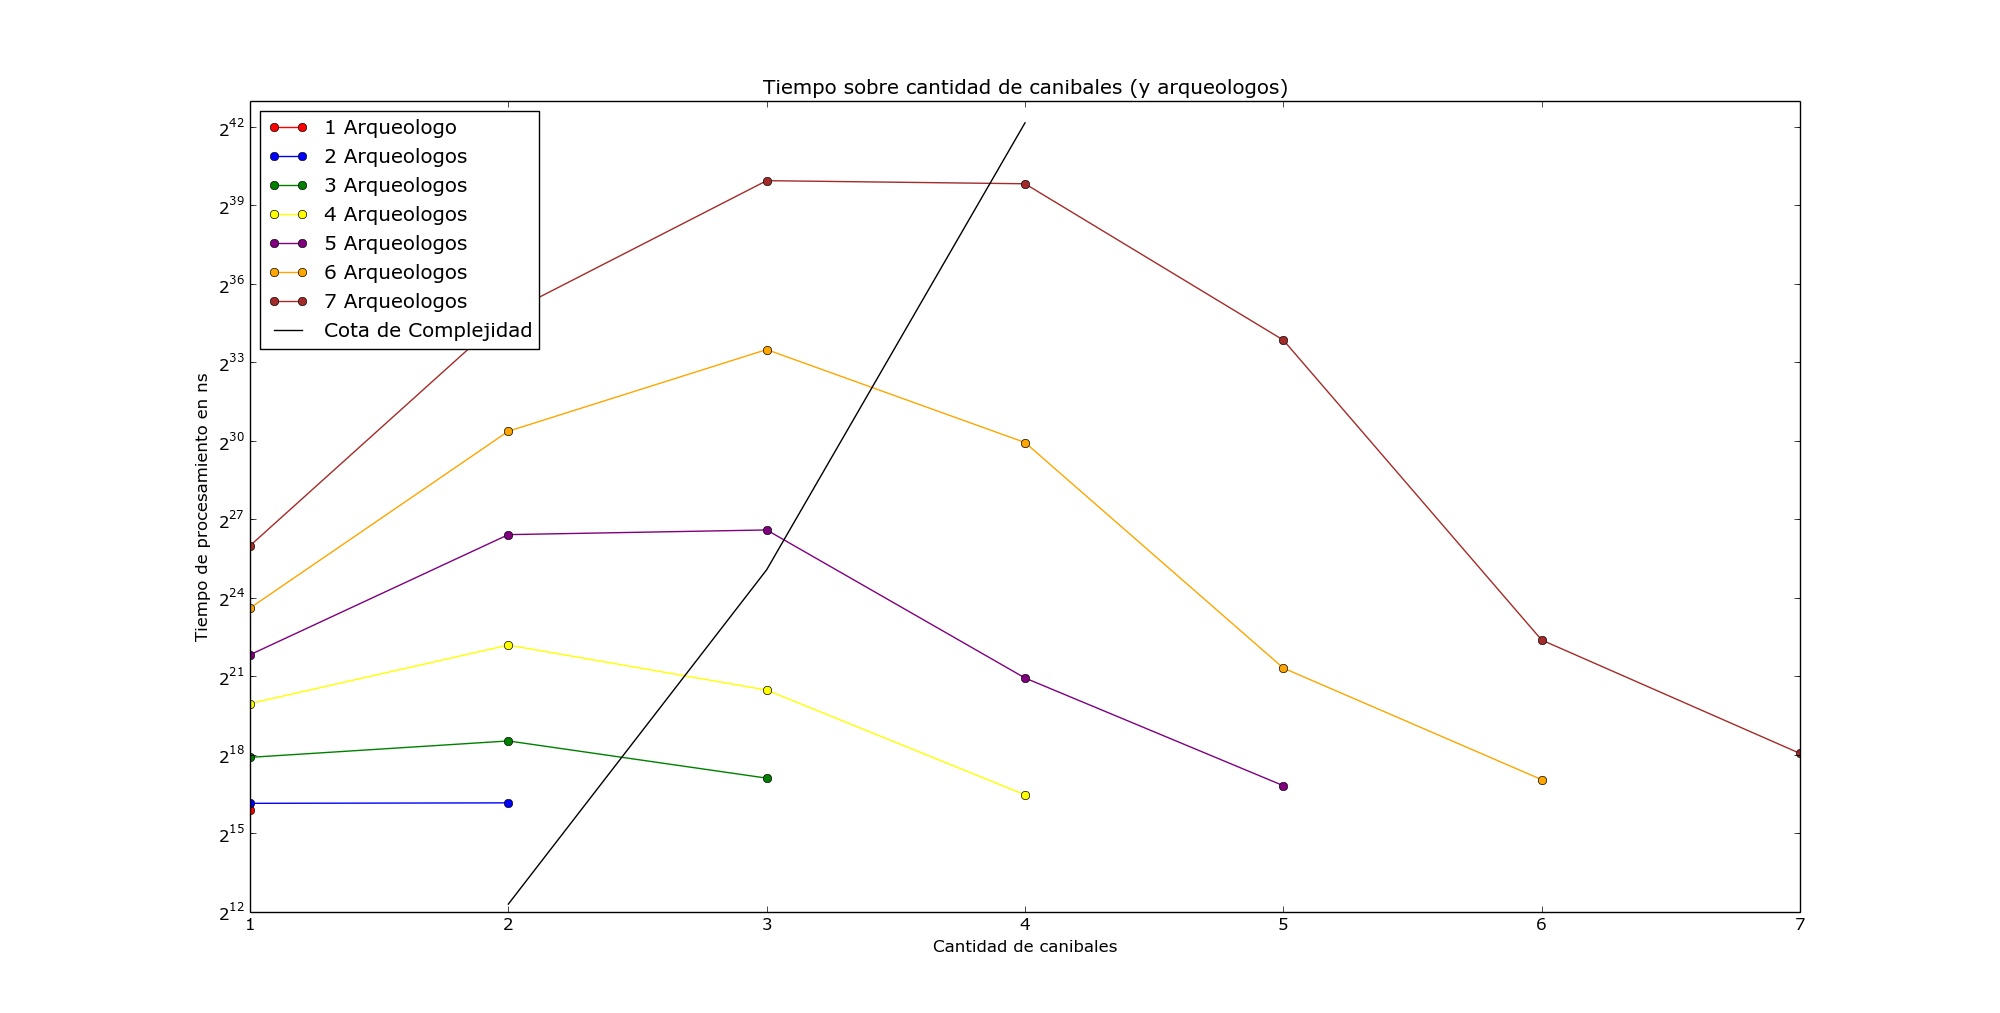
\includegraphics[scale=0.25]{imagenes/ej1Nuevo.jpeg}
        \caption{}
      \end{center}
  \end{figure}

  Pudimos notar como la cota de complejidad efectivamente cumple su propósito a pesar de que tiene un crecimiento completamente distinto al del algoritmo. Los peores casos encontrados se mantuvieron entre 2 y 3 caníbales para los 7 casos de arqueólogos. Entre 0 y ellos, el crecimiento se asemeja a la función de cota propuesta.
  Evidentemente, lo que pasaba era que a partir de cierta cantidad de caníbales y arqueólogos, el algoritmo encontraba de manera más rápida que no había forma de que crucen todos los arqueólogos y se salven.

  COMPLETAR?!?!?!?!?!?!?!?!?
  COMPLETAR?!?!?!?!?!?!?!?!?
  COMPLETAR?!?!?!?!?!?!?!?!?
  COMPLETAR?!?!?!?!?!?!?!?!?

  Para el caso en que no haya arqueólogos y solo haya caníbales, esperábamos que la resolución del problema sea más rápida que en los casos que hay más arqueólogos que caníbales. Probamos con cantidades de caníbales entre 1 y 200 y en el próximo grafico se ilustran los resultados de tiempo en función del número de personas.

  \begin{figure}[H]
      \begin{center}
        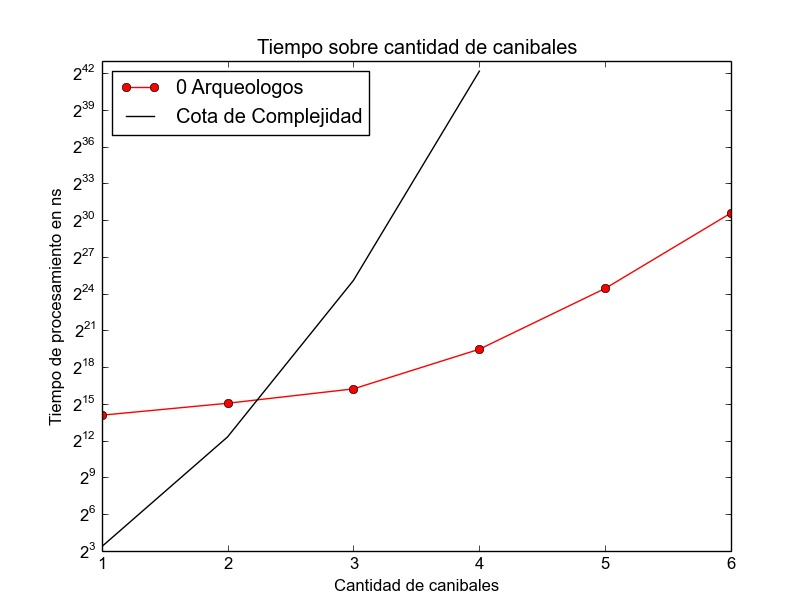
\includegraphics[width=0.7\columnwidth]{imagenes/ej1exp2NuevaVersion.jpeg}
        \caption{}
      \end{center}
  \end{figure}

  Notamos como el tiempo que toma a mayor cantidad de caníbales sin arqueólogos crece mucho más lento que para los casos con arqueólogos. Esto se debe a que las ramas en que cruzan arqueologos no se prueban, sino que solo se intenta que crucen 1 o 2 caníbales. Luego, la cantidad de estados posibles se reduce a 2 veces la cantidad de formas que se pueden distribuir los caníbales en ambos lados del puente (una por cada lado de la linterna), que es igual a $2*(n^2)$; reducimos la cota de complejidad a $O(n^2*2^{n^2})$. El cambio no es muy grande debido a que las cotas no están totalmente ajustadas, pero funcionan para dar una idea del peor caso acotado por arriba.
